\chapter{Implementation}

This chapter describes \ldots compares \ldots




\section{Artoo}

Artoo consists of a general-purpose {\tt SVGGraph}  -- and a


\section{Experimental methodology}


\subsection{Test data}

\begin{itemize}
    \item Four graphs from \citet{aldenthesis}
\end{itemize}

Up to a point, GSN arguments are quite homogeneous. 


\section{Springy}

Springy.js is an existing JavaScript implementation of a force directed graph drawing algorithm.
It lays out graphs by representing nodes as point charges and edges as springs. Springy.js simulates the electrostatic forces of interaction between these point charges, and the extension of the springs caused by these forces, according to Coulomb's and Hooke's laws.

\subsection{Hooke's law}

Hooke's law describes the relationship between the force exerted on a spring, and the distance by which it extends as a result of that force being exerted.
It states that the distance is proportional to the force:

$$
F = -kX
$$

(where $F$ is the force exerted on the spring, $X$ is the distance by which it extends, and $k$ is a constant representing the spring's stiffness)

\subsection{Coulomb's law}

Coulomb's law describes the electrostatic force of interaction between two point charges.

``is directly proportional to the scalar multiplication of the magnitudes of charges and inversely proportional to the square of the distance between them.''

``The force is along the straight line joining them. If the two charges have the same sign, the electrostatic force between them is repulsive; if they have different sign, the force between them is attractive.'' \todo{reference}

In scalar form:

$$
|\mathbf F|=k_e{|q_1q_2|\over r^2}\qquad
$$

(where $F$ F is the $q_1$ and $q_2$ are the two charges, $r$ is the distance between them, and $k_e$ is Coulomb's constant 

In vector form:

$$
\qquad\mathbf F_1=k_e\frac{q_1q_2}{{|\mathbf r_{21}|}^2} \mathbf{\hat{r}}_{21},\qquad
$$


Coulomb's law closely resembles Newton's law of universal gravitation, which describes the gravitational force between two masses.
But gravitational force is always attractive (if it is assumed that nothing can have negative mass), whereas the electrostatic force described by Coulomb's law can be repulsive (if both particles' charges have the same sign).

\subsection{Newton's laws of motion}

Newton's three laws of motion are also relevant to a force directed layout.

\subsection{Implementing }

Springy, as distributed [online], consists of a layout algorithm implemented in JavaScript (springy.js) along with a sample renderer for displaying a graph layout.

\section{Arbor}

Simple though the brute-force force directed algorithm implemented in Springy is to understand, it also inefficient.

The Barnes-Hut algorithm is $O$



\section{Dagre}

An key part of the layered layout approach is notion that directed graphs flow in a single direction (typically from top to bottom or from left to right). This is highly applicable to GSN arguments, particularly as specified by the GSN community standard document's guidelines \cite{gsnspec} (see

Figure~\ref{fig:dagre1} shows

\begin{figure}
  \centering
  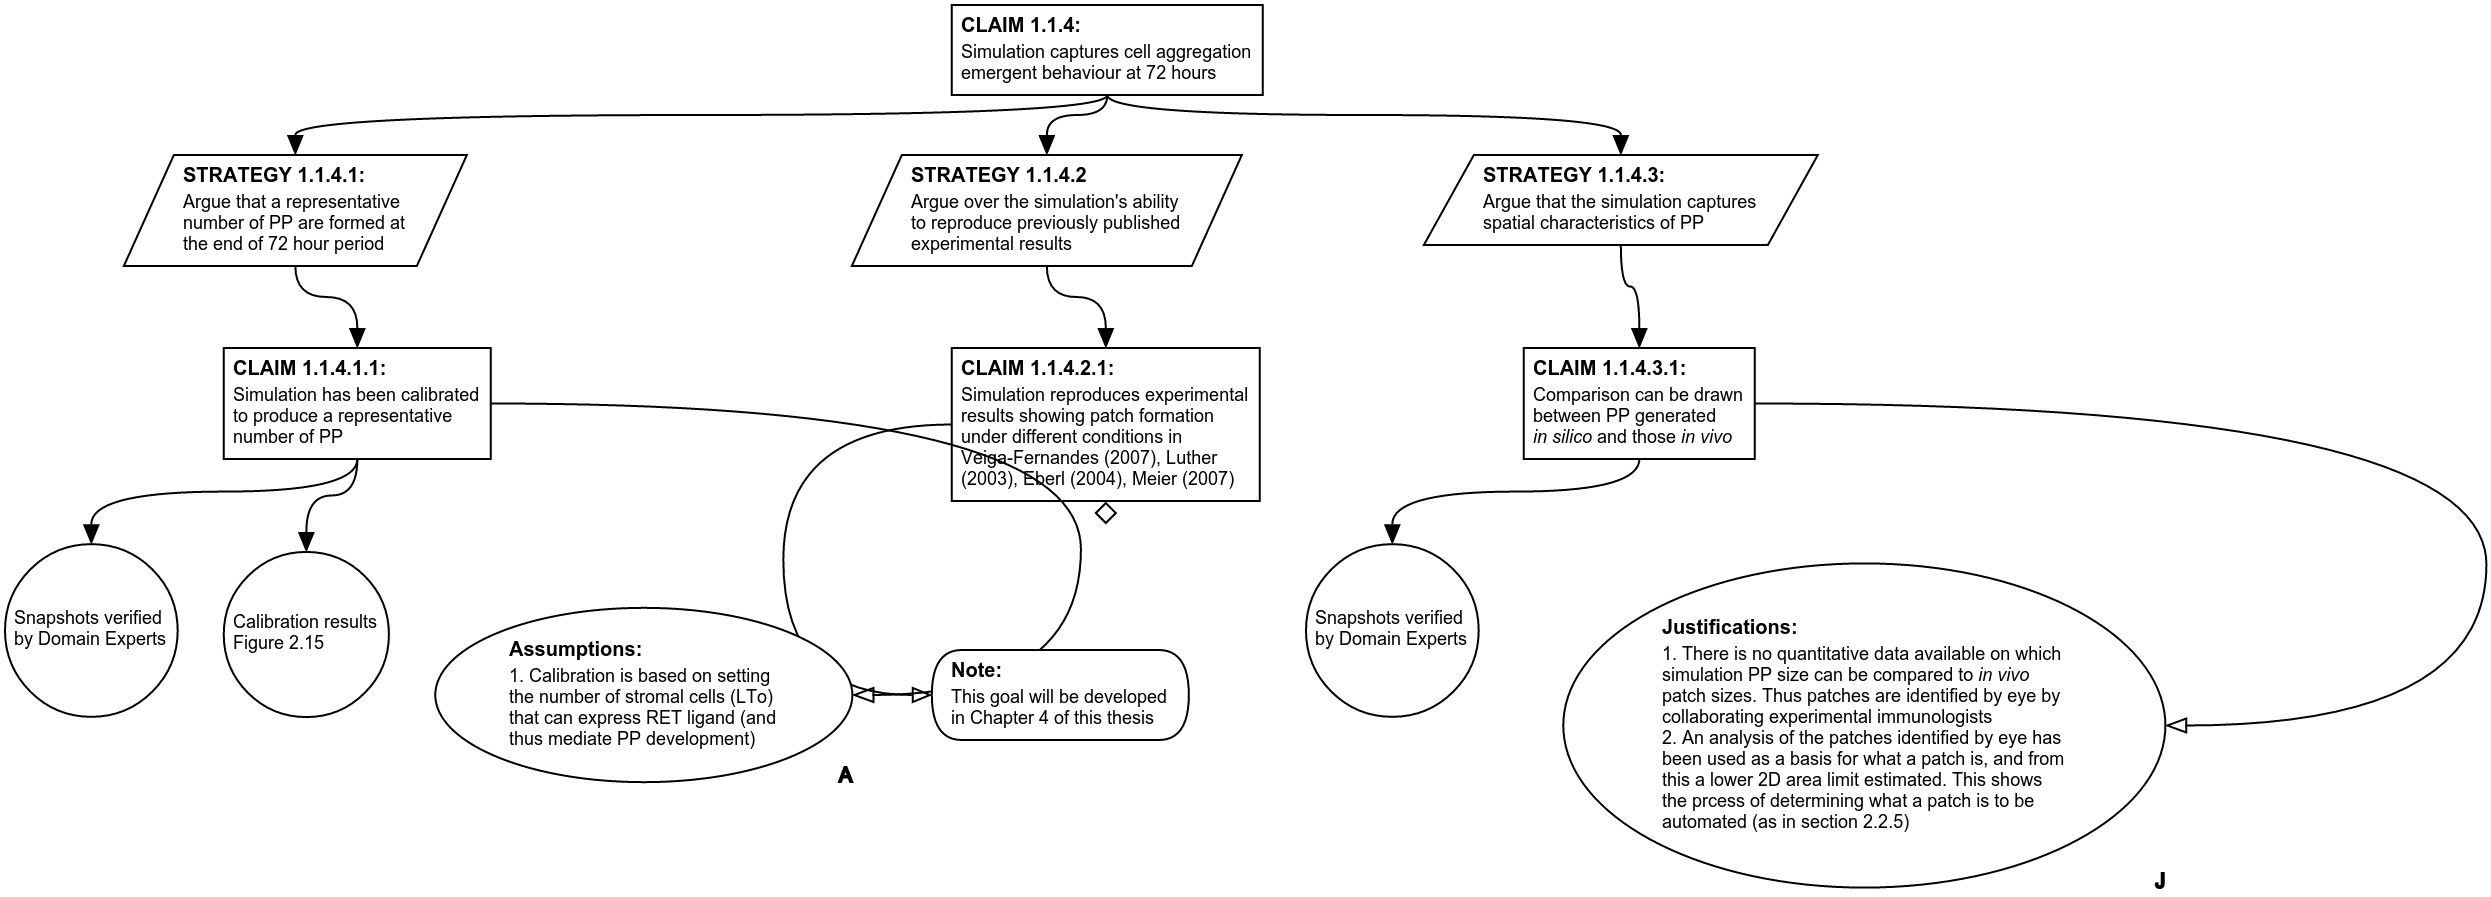
\includegraphics[width=\textwidth]{graphics/results/dagre.png}
  \label{fig:dagre1}
\end{figure}



\begin{figure}
  \centering
  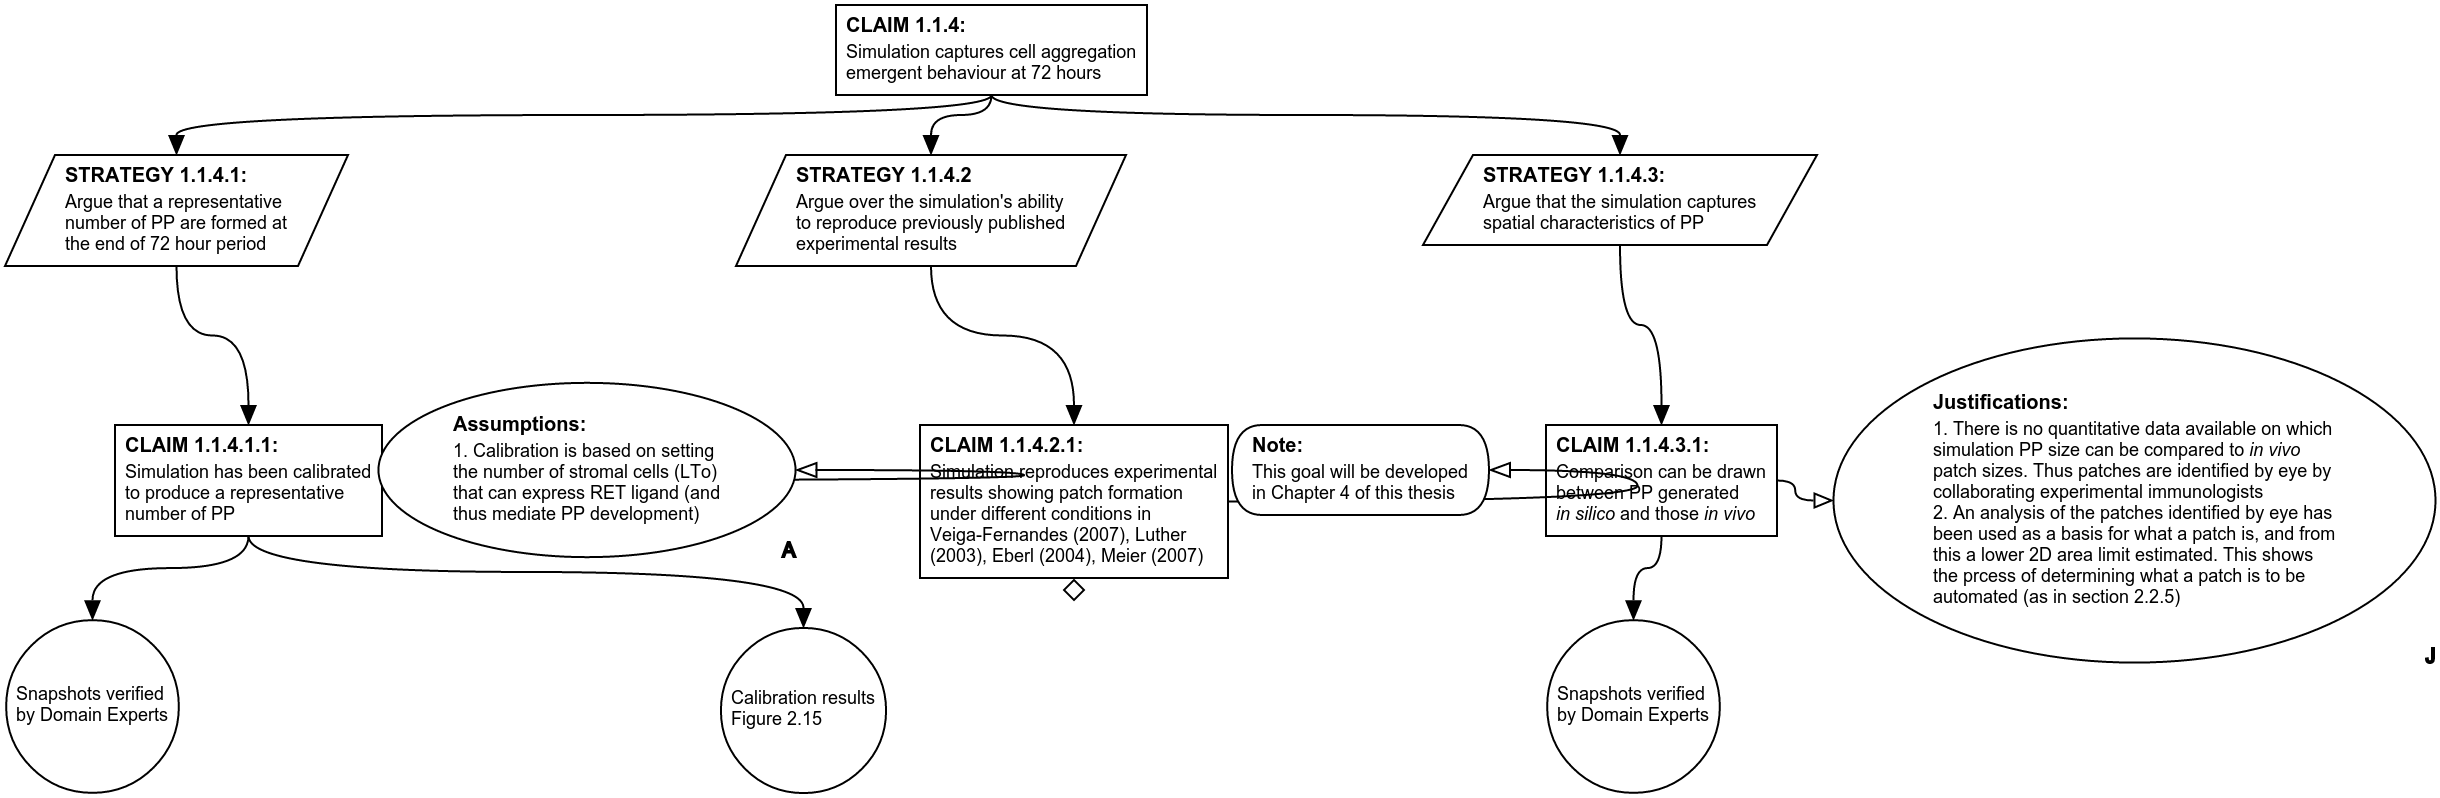
\includegraphics[width=\textwidth]{graphics/results/dagre-enhanced.png}
  \caption{A less naive use of Dagre, with InContextOf connections 
  \label{fig:dagre2}
\end{figure}



\begin{landscape}

\section{Testing}



\subsection{Results}

\subsubsection{Dagre}

\begin{tabular}{ | c | c | c | c | }
    \hline
    Graph & Area & Running time & Edge crossings \\
    \hline
    1     & & & \\
    \hline
    2     & & & \\
    \hline
    3     & & & \\
    \hline
    4     & & & \\
    \hline
\end{tabular}



\end{landscape}